% RESULTS CHAPTER
\chapter{Results}\label{ch:results}

In this chapter, the performance of the prediction model is analysed, and the discussion of the results are explored.
The machine learning algorithms are evaluated to determine the best model at predicting on unknown data.

\section{Performance Metrics}\label{sec:Performance Metrics}

The performance of any algorithm is evaluated by a few factors that are measured on the test dataset, where the trained model attempts to correctly predict the target field and this performance is then compared to its true outcome.
This assessment method is the norm on any binary classification problem and often will be visualised using a confusion matrix.
The confusion matrix is a simple visualisation in which the four possible permutations of predictions are displayed.
As seen in Figure~\ref{fig:ConfusionMatrix10}, it compares the number of predictions of wins and losses made by the model versus the number of real wins and losses found in the dataset. \\

\begin{figure}[h]
    \centering
    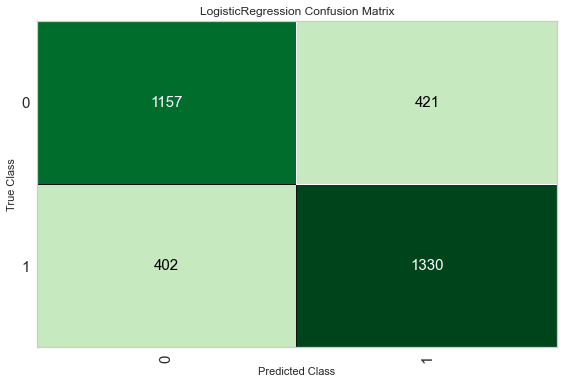
\includegraphics[width=0.8\textwidth]{figures/ConfusionMatrix10}
    \caption{A confusion matrix of a Logistic Regression Model trained on the 10 minute dataset}
    \label{fig:ConfusionMatrix10}
\end{figure}

On the y-axis the true class of the result can be seen, and on the x-axis there is the model's predicted class.
These four possible permutations are commonly referred to as follows:
\begin{itemize}
    \item \ac{TP} is seen in the bottom right of the matrix, this is when the predicted win actually reflects the true win.
    \item \ac{TN} is seen in the top left of the matrix, this is when the predicted loss actually reflects the true loss.
    \item \ac{FP} is seen in the top right of the matrix, this is when the predicted win is incorrect and the true class is a loss.
    \item \ac{FN} is seen in the bottom left of the matrix, this is when the predicted loss is incorrect and the true class is a win.
\end{itemize}

By collecting these outcome values, the effectiveness of each model is then able to be assessed via many performance metrics that are calculated using these values.
These measures each give an understanding of a model, with different implications depending on the objective of the project being assessed.
In this study, the focus is on assessing the correct classifications and there is little to no consequences for misclassification.
Therefore, the main criteria needed are the proportion of true classifications - aka the number of \ac{TP}s and \ac{TN}s compared to the whole prediction group.
This calculation is also known as the Accuracy of the prediction, and is calculated as follows:

\[ Accuracy = \frac{\sum TP + \sum TN}{\sum TP + \sum TN + \sum FP + \sum FN} \]

This is considered the key metric for this problem, as our dataset is pretty balanced so the other metrics such as Precision and Recall are not as important.
Here Accuracy can help decide how well a given model is predicting the correct outcomes of an esports League of Legends match.
The Accuracy of a model is only an effective metric if higher than the balance of the dataset, thus must be greater than 52.8\% to show any improvement over guessing the balance of the data.
Other metrics such as AUC, Precision, Recall are also calculated and evaluated, these metrics are calculated as such:

\begin{gather*}
    Precision = \frac{\sum TP}{\sum TP + \sum FP}\\
    Recall = \frac{\sum TP}{\sum TP + \sum FN}\\
    FPR = \frac{\sum FP}{\sum FP + \sum TN}\\
\end{gather*}

A \ac{ROC} curve is a graph that plots the Recall versus the \ac{FPR}, it plots these performance metrics between the bounds of zero and one.
\ac{AUC}, is a measure that understandably calculates the area under the \ac{ROC} curve which provides a measure of performance across all possible classification thresholds~\citep{aucGoogle}.
Essentially, \ac{AUC} is the probability that a model can distinguish between a positive and negative class - in this study it represents the ability to distinguish wins from losses.
Therefore, to conclusively accept a model as a feasible option, the Accuracy and AUC are the two core metrics that a model will have to score sufficiently on and will ultimately be the performance indicators to evaluate with. \\


\section{Model Results}\label{sec:Model Results}
\subsection{10 Minute Model}\label{subsec:10-minute-model}


As seen in Table~\ref{tab:ModelResults10}, most of the machine learning algorithms score quite similarly.
The four metrics of Accuracy, AUC, Recall and Precision all are within a 5\% range for every algorithm tested.
Here the best performing machine learning algorithm is the Logistic Regression model, scoring an accuracy of 75.06\% and an AUC of 82.30\%.
This is closely followed by the Linear Discriminant Analysis at an identical accuracy, but with an AUC of 82.28\%. \\

\begin{table}[h!]
    \centering
    \caption{A table showing the model results for the 10 minute dataset}
    \begin{tabular}{l c c c c }
        \toprule
        \textbf{Model} & \textbf{Accuracy} & \textbf{AUC} & \textbf{Recall} & \textbf{Precision} \\
        \midrule
        Logistic Regression & 0.7506 & 0.8230 & 0.7798 & 0.7574  \\
        Linear Discriminant Analysis & 0.7506 & 0.8228 & 0.7813 & 0.7566 \\
        Ada Boost Classifier & 0.7469 & 0.8181 & 0.7747 & 0.7546 \\
        Naive Bayes & 0.7458 & 0.8128 & 0.7613 & 0.7599 \\
        Gradient Boosting Classifier & 0.7458 & 0.8407 & 0.7759 & 0.7529 \\
        Quadratic Discriminant Analysis & 0.7456 & 0.8363 & 0.7601 & 0.7604 \\
        SVM - Linear Kernel & 0.7436 & 0.0000 & 0.7769 & 0.7492 \\
        Light Gradient Boosting Machine & 0.7357 & 0.8316 & 0.7630 & 0.7453 \\
        Random Forest Classifier & 0.7316 & 0.8230 & 0.7498 & 0.7462 \\
        Extra Trees Classifier & 0.7248 & 0.8116 & 0.7459 & 0.7385  \\
        K Neighbors Classifier & 0.7061 & 0.7794 & 0.7276 & 0.7212  \\
        Decision Tree Classifier & 0.6804 & 0.6794 & 0.6969 & 0.6998 \\
        \bottomrule
    \end{tabular}
    \label{tab:ModelResults10}
\end{table}

Interestingly enough the decision tree based algorithms that were commonly used in previous studies such as Random Forest, appear to perform slightly worse than algorithms such as Logistic Regression or Linear Discriminant Analysis.
These techniques are techniques based on linear regression analysis that opt to find a linear combination of features that cause separation in a problem.
These results then may indicate that the problem of match outcomes in League of Legends is linearly separable.
The model for the 10-minute mark was chosen to be built upon a logistic regression technique.
Firstly, the model is tested across the data split by the stratified k-fold cross-validation and tuned afterwards.
The resultant performance metrics can be seen in Table~\ref{tab:Kfold10}. \\

\begin{table}[h]
    \centering
    \caption{A table showing the mean metrics for the 10 minute logistic regression model after 10-fold cross-validation}
    \begin{tabular}{lcccccc}
        \toprule
        \textbf{} & \textbf{Accuracy} & \textbf{AUC} & \textbf{Recall} & \textbf{Precision} \\
        \midrule
        Mean & 0.7516 & 0.8226 & 0.7618 & 0.7682 \\
        Std & 0.0150 & 0.0169 & 0.0285 & 0.0116 \\
        \bottomrule
    \end{tabular}
    \label{tab:Kfold10}
\end{table}

Table~\ref{tab:Kfold10} shows very similar results to the previous stated values, meaning that the model tuning had very little effect on improving the model's performance.
It also gives a standard deviation on the core metrics of under 2\%.
During the modelling, the feature importance of the features included in the dataset were calculated.
Figure~\ref{fig:FeatureImport10} shows the average relative importance of each feature when using the 10-minute dataset.
The top 10 features by feature importance are presented down the y-axis in decreasing order according to their relative importance values.
The most important features are those related to the player performance inside their lanes such as `csdiffat10', `deathsat10' and `KillParat10', with more objective team-based features having lower importance in predicting the resultant outcome of a given match.
At first this seems counter-intuitive, especially when given that teams must destroy towers in order to eventually win the game.
However, it is likely that at this stage of the game there is very low likelihood that teams can effectively destroy towers, so the focus should be on progressing their individual leads inside their lane.
These leads that they garner are reflected in the three features mentioned previously, and should translate into further advantages in more objective oriented features in a later game-state. \\

\begin{figure}[h]
    \centering
    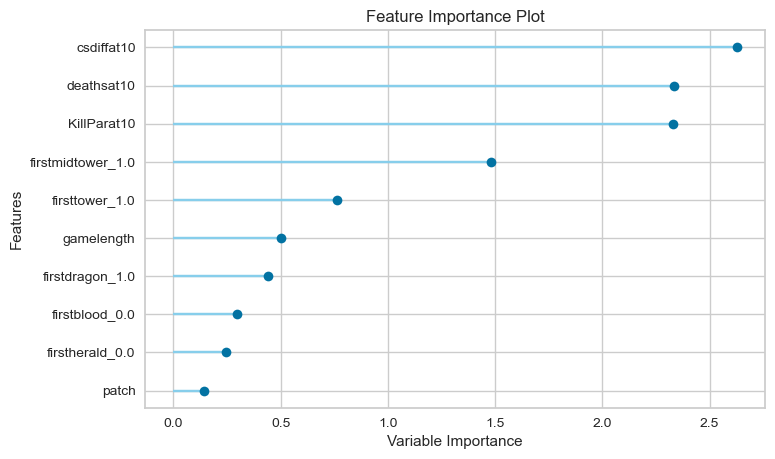
\includegraphics[width=\textwidth]{figures/FeatureImport10}
    \caption{A graph showing the Relative Importance of the features in the Logistic Regression Model using the 10 minute dataset}
    \label{fig:FeatureImport10}
\end{figure}

\newpage

\subsection{15 Minute Model}\label{subsec:15-minute-model}

Table~\ref{tab:ModelResults15} highlights that once again that all but one of the machine learning algorithms score within a 5\% range of the four key metrics tracked.
The two best performing machine learning algorithm remain the Logistic Regression model and the Linear Discriminant Analysis model, scoring an accuracy of 76.84\% and 76.87\%,  and AUC values of 84.74\% and 84.53\% respectively.
Once again the decision tree based algorithms that were commonly used in previous studies appear to vastly under-perform when compared to Logistic Regression or Linear Discriminant Analysis, with the Decision Tree Classifier falling behind by roughly 10\% across all the four key metrics calculated.
It is once again chosen for the Logistic Regression model to be the final model for the 15-minute dataset.
The model is once again built and a stratified k-fold cross-validation is applied.
The final performance metrics can be seen in Table~\ref{tab:Kfold15}. \\

\begin{table}[h]
    \centering
    \caption{A table showing the model results for the 15 minute dataset}
    \begin{tabular}{l c c c c }
        \toprule
        \textbf{Model} & \textbf{Accuracy} & \textbf{AUC} & \textbf{Recall} & \textbf{Precision} \\
        \midrule
        Linear Discriminant Analysis & 0.7687 & 0.8453 & 0.7994 & 0.7727 \\
        Logistic Regression & 0.7684 & 0.8474 & 0.7972 & 0.7733  \\
        Ridge Classifier & 0.7681 & 0.0000 & 0.7986 & 0.7721  \\
        Ada Boost Classifier & 0.7662 & 0.8418 & 0.7899 & 0.7741   \\
        Quadratic Discriminant Analysis & 0.7643 & 0.8578 & 0.7794 & 0.7772  \\
        Gradient Boosting Classifier & 0.7638 & 0.8601 & 0.7935 & 0.7690  \\
        Naive Bayes & 0.7589 & 0.8362 & 0.7694 & 0.7746  \\
        Light Gradient Boosting Machine & 0.7577 & 0.8551 & 0.7877 & 0.7635  \\
        SVM - Linear Kernel & 0.7562 & 0.0000 & 0.7835 & 0.7642 \\
        Random Forest Classifier & 0.7519 & 0.8483 & 0.7745 & 0.7623  \\
        Extra Trees Classifier & 0.7431 & 0.8359 & 0.7652 & 0.7545  \\
        K Neighbors Classifier & 0.7307 & 0.8067 & 0.7449 & 0.7470  \\
        Decision Tree Classifier & 0.6870 & 0.6854 & 0.7125 & 0.7021  \\
        \bottomrule
    \end{tabular}
    \label{tab:ModelResults15}
\end{table}

Table~\ref{tab:Kfold15} shows an accuracy increase of 0.22\% after tuning, bumping the Logistical Regression model accuracy value to 77.06\%.
The change in the accuracy of the model between the 10 to 15 minute models only increases by roughly 2\%.
This increase is much lower than expected when compared to previous studies such as~\citet{silva2018continuous, lee2020predicting} achieving increases of ~5-6\% between the same period in game time, albeit whilst achieving accuracy levels on par or greater than its predecessors.
These differences between studies are likely due to differences in the feature selection stage, as well as both the quality of the data collected and the metrics that the data offer.
In the dataset used in this study, there are many binary objective-type features that are labelled as to which team had completed them first.
These variables are often important milestones that help a team towards victory throughout the game, but most importantly they often can reveal which team is in control at a given game-time and thus be a key predictor into the victor of the overall match. \\

\begin{table}[h]
    \centering
    \caption{A table showing the mean metrics for the 15 minute Logistic Regression model after 10-fold cross-validation}
    \begin{tabular}{lcccccc}
        \toprule
        \textbf{} & \textbf{Accuracy} & \textbf{AUC} & \textbf{Recall} & \textbf{Precision} \\
        \midrule
        Mean & 0.7706 & 0.8478 & 0.7752 & 0.7889 \\
        Std & 0.0200 & 0.0173 & 0.0289 & 0.0198 \\
        \bottomrule
    \end{tabular}
    \label{tab:Kfold15}
\end{table}

Again, the feature importance of the features included in the dataset were calculated and visualised.
Figure~\ref{fig:FeatureImport15} shows the average relative importance of each feature when using the 15-minute dataset.
It remains that the most important features are those related to the player performance inside their lanes such as `csdiffat15', `deathsat15' and `KillParat15', with slightly more emphasis on `deathsat15' when compared to the previous model.
In fact the relative importance for these features has roughly doubled
with more objective team-based features having lower importance in predicting the resultant outcome of a given match.
An interesting feature that appears here is in fact when the blue side team loses their first tower.
The model believes this to be an important factor in the blue side achieving a victory, which is the opposite notion to what the previous model suggests.
However, the model still believes that destroying the mid-lane tower is the prime team-based objective on the map within the first 15 minute mark.
This could lead to the conclusion that as long as the blue side team obtains the first mid-lane tower, but allows the opposition to take the first tower in either the top or bottom lane, that this will still lead to a higher probability of a match victory. \\


\begin{figure}[h]
    \centering
    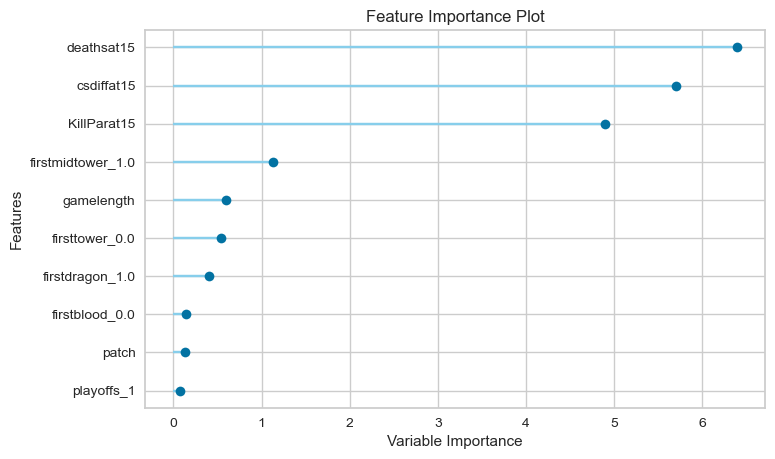
\includegraphics[width=0.8\textwidth]{figures/FeatureImport15}
    \caption{A graph showing the Relative Importance of the features in the Logistic Regression Model using the 15 minute dataset}
    \label{fig:FeatureImport15}
\end{figure}

\newpage

\subsection{20 Minute Model}\label{subsec:20-minute-model}

Again all the machine learning algorithms score within a performance metric range of 5\% as seen in Table~\ref{tab:ModelResults20}.
This just reiterates that there is minimal difference in performance between the machine-learning algorithms tested, with the decision tree based algorithms generally falling behind.
This remains true aside from the Gradient Boosting Classifier, where it is in-fact the best performing model overall.
It scored an accuracy of 85.85\% and an AUC of 94.33\%.
It was then closely followed by the two previous algorithms mentioned in both Section~\ref{subsec:10-minute-model} and~\ref{subsec:15-minute-model} - the Logistic Regression and the Linear Discriminant Analysis at identical accuracies of 85.83\%, but with respective AUC values of 92.66\% and 92.57\%.
This sequential increase of accuracy in the models reinforces Hypothesis 1, suggesting that prediction accuracy would increase in proportion to the gamelength.
However the machine learning algorithm results seem to reject the claim made in Hypothesis 3, as when compared to other algorithms such as the Linear Discriminant Analysis or Logistic Regression, the decision tree-based algorithms tend to be weaker predictors of match outcomes. \\

\begin{table}[h]
    \centering
    \caption{A table showing the model results for the 20 minute dataset}
    \begin{tabular}{l c c c c }
        \toprule
        \textbf{Model} & \textbf{Accuracy} & \textbf{AUC} & \textbf{Recall} & \textbf{Precision} \\
        \midrule
        Gradient Boosting Classifier & 0.8585 & 0.9433 & 0.8782 & 0.8586  \\
        Logistic Regression & 0.8583 & 0.9266 & 0.8648 & 0.8679 \\
        Linear Discriminant Analysis & 0.8583 & 0.9257 & 0.8513 & 0.8780 \\
        Quadratic Discriminant Analysis & 0.8582 & 0.9406 & 0.8706 & 0.8634 \\
        Ridge Classifier & 0.8581 & 0.0000 & 0.8511 & 0.8778 \\
        Ada Boost Classifier & 0.8559 & 0.9245 & 0.8623 & 0.8655 \\
        Random Forest Classifier & 0.8525 & 0.9387 & 0.8653 & 0.8581 \\
        SVM - Linear Kernel & 0.8521 & 0.0000 & 0.8504 & 0.8701 \\
        Light Gradient Boosting Machine & 0.8494 & 0.9392 & 0.8645 & 0.8538  \\
        Extra Trees Classifier & 0.8451 & 0.9315 & 0.8584 & 0.8512 \\
        K Neighbors Classifier & 0.8367 & 0.9057 & 0.8433 & 0.8482 \\
        Naive Bayes & 0.8284 & 0.9122 & 0.8509 & 0.8300 \\
        Decision Tree Classifier & 0.8024 & 0.8017 & 0.8140 & 0.8137\\
        \bottomrule
    \end{tabular}

    \label{tab:ModelResults20}
\end{table}

For this model, the Gradient Boosting Classifier is chosen as it scores high on all major performance metrics calculated.
After the model is tuned, the accuracy increases to 85.99\%, an increase of 0.14\% - see Table~\ref{tab:Kfold20}.
The change in the accuracy of the model between the 10 to 15 minute models only increases by roughly 2\%.
From the previous model, the accuracy increases
This is much lower than expected when compared to previous studies such as~\citet{silva2018continuous, lee2020predicting} achieving increases of ~5-6\% between the same period in game time, albeit whilst achieving accuracy levels on par or greater than its predecessors. \\

\begin{table}[h]
    \centering
    \caption{A table showing the mean metrics for the 20 minute Gradient Boosting Classifier model after 10-fold cross-validation}
    \begin{tabular}{lcccccc}
        \toprule
        \textbf{} & \textbf{Accuracy} & \textbf{AUC} & \textbf{Recall} & \textbf{Precision} \\
        \midrule
        Mean & 0.8599 & 0.9433 & 0.8789 & 0.8602 \\
        Std & 0.0061 & 0.0042 & 0.0130 & 0.0087 \\
        \bottomrule
    \end{tabular}

    \label{tab:Kfold20}
\end{table}

The average relative importance for the Gradient Boosting Classifier model is shown in Figure~\ref{fig:FeatureImport20}.
Now at the 20 minute mark the features that are most influential inside the model have changed.
Suddenly the player performance features that were dominating the relative importance previously such as `csdiffat15', `deathsat15' and `KillParat15' have now fallen out of favour versus the team-based map objectives.
Here the `firstbaron' metric becomes the focal feature in whether a team will achieve the victory, with a relative importance three times as large as the next highest.
The next two key features are `gamelength' and `firsttothreetowers', reiterating the
team-based map objectives being key to achieving victory as the gamelength increases.
The `firstbaron' feature being this impactful makes logical sense when accounting for the context behind the powerful \gls{buff} that this monster grants when slain.
This \gls{buff} gives players the ability to increase the power of their surrounding \glspl{minion}, and thus a large increase in the capability to destroy enemy \glspl{tower} or \glspl{inhibitor}.
Subsequently, the team that slays the \gls{baron} is granted a large sum of experience and gold through the monster itself, as well as the towers that could also fall.
This large spike in income and champion strength likely  helps the team to win future fights and then the match, this snowballing effect was hypothesised in Hypothesis 1 during Chapter~\ref{ch:literaturereview}. \\

\begin{figure}[h]
    \centering
    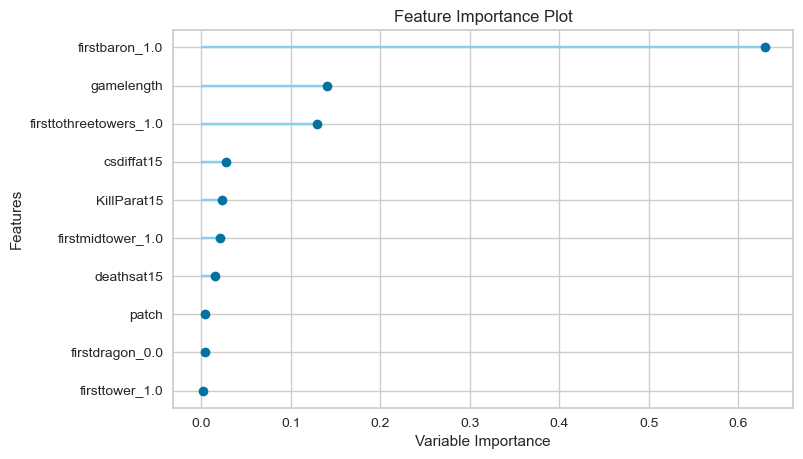
\includegraphics[width=0.8\textwidth]{figures/FeatureImport20}
    \caption{A graph showing the Relative Importance of the features in the Gradient Boosting Classifier Model using the 20 minute dataset}
    \label{fig:FeatureImport20}
\end{figure}


\section{Discussion of Results}\label{sec:discussion-of-results}

The results of these three models indicate that there is potential for a highly efficient League of Legends esports prediction model.
Using a mixture of Logistic Regression models and Gradient Boosting Classifiers the accuracy of predictions were calculated between the 10 to 20 in-game minute mark.
A summary of these results can be seen in Table~\ref{tab:ModelCompare}. \\

\begin{table}[h]
    \centering
    \caption{A table comparing the performance metrics for all three models}
    \begin{tabular}{lcccc}
        \toprule
        \textbf{Model} & \textbf{Accuracy} & \textbf{AUC} & \textbf{Recall} & \textbf{Precision} \\
        \midrule
        10 Minute LR & 0.7516 & 0.8226 & 0.7618 & 0.7682 \\
        15 Minute LR & 0.7706 & 0.8478 & 0.7752 & 0.7889 \\
        20 Minute GBC & 0.8599 & 0.9433 & 0.8789 & 0.8602 \\
        \bottomrule
    \end{tabular}
    \label{tab:ModelCompare}
\end{table}

The assumption can be made that with no prior knowledge any given League of Legends esports match result can be roughly predicted via coinflip, with the class balance shown previously in Figure~\ref{fig:DataBalance}.
However using the models create in this study, an average layman could theoretically predict the match outcome over 75\% of the time when given some key features at the 10 minute mark, with this increasing to 86\% by the 20 minute mark.
Using the key figures seen in Table~\ref{tab:ModelCompare}, it can be seen that when compared to previous attempts at a similar form of prediction modelling for League of Legends, these models exceed the metrics found by many of its predecessors. \\

\citet{silva2018continuous} used \ac{RNN}s for their prediction modelling using esports data between 2015 and early 2018, similar to this study they produced results for time intervals during the game.
\citet{lee2020predicting} used a Random Forest Classifier for their modelling using ranked data extracted from the Riot API, and once again produced results for varying time intervals in-game.
The results published in those studies have been collated into Table~\ref{tab:LitCompare}.
Here it can be seen that the prediction accuracy is much higher than those stated in previous studies, with improvements up to ~7\% at the 10 minute interval.
This means that the models created during this study not only contribute more proof to the growing numbers of literature surrounding predictive modelling in the esports industry, but are also outperforming the most recent literature in the field.
As seen with all the results collated, the improvements to the prediction accuracy increases as the in-game timer increases.
All three studies show an accuracy increase of 10\% from the 10 minute mark to the 20 minute mark, regardless of the initial accuracy.
This reaffirms Hypothesis 1 stated in Section~\ref{sec:Summary}, ultimately verifying the idea that a match of League of Legends has a snowballing nature, thus the outcome becomes more predictable as it progresses.
Hypothesis 2 can generally be assumed to be true when looking at the correlations between many of the features during the data exploration phase, these correlation values are highlighted in Figure~\ref{ch:Feature Correlations}.
Many of these features have a correlation level between 0.4 and 0.8, which suggests a moderate to strong level of correlation and can lead the overall model to suffer from some level of multicollinearity.
The best performing models in this study were the Logistic Regression and the Gradient Boosting Classifier, with the Logistic Regression being used for two of three models.
Hypothesis 3 stated that a decision tree algorithm will likely be the optimal algorithm for the prediction model, but this ultimately was proven to be mostly wrong with the exception of the Gradient Boosting Classifier.

\begin{table}[h]
    \centering
    \caption{A table comparing the accuracy for different time intervals from other studies~\citep{silva2018continuous, lee2020predicting}}
    \begin{tabular}{lccc}
        \toprule
        \textbf{Study} & \textbf{10 Minutes} & \textbf{15 Minutes} & \textbf{20 Minutes} \\
        \midrule
        This Study & 0.7516 & 0.7706 & 0.8599  \\
        Silva et al. & 0.6869 & 0.7523 & 0.8018 \\
        Lee et al. & 0.6788 & 0.7318 & 0.7649  \\
        \bottomrule
    \end{tabular}
    \label{tab:LitCompare}
\end{table}